\documentclass[journal]{IEEEtran}
\usepackage{graphicx}
\usepackage{caption}
\usepackage{hyperref}

\begin{document}
\title{VITAL: What is in Your Code? \protect\\  A Survey Addressing the Growth and Risks of Using Third-Party Dependencies}

\author{
\IEEEauthorblockN{Thomas G. Hastings\IEEEauthorrefmark \protect\\}
%\vspace{0.05in}
\IEEEauthorblockA{University of Colorado at Colorado Springs  \protect\\ \emph{thasting@uccs.edu}}
%\vspace{0.05in}
}

% The paper headers
\markboth{VITAL: What is in Your Code? A survey addressing the growth and risks of using third-party dependencies}%
{Shell}

% make the title area
\maketitle
\begin{abstract}
Software developers have become increasingly dependent on open source software dependencies as they work to develop software systems. Often, developers bring in open source dependencies through convenient package managers without thinking about the risk they may be exposing their organization to. In this paper we will survey three main topics related to  open source package adoption, package management, and how to manage some of the risk posed by open source packages using the VITAL technique. 
\end{abstract}

\begin{IEEEkeywords}
Software Engineering, Dependency Management, Open Source Software, Secure Software Engineering
\end{IEEEkeywords}

\section{Introduction}
% Some journals put the first two words in caps:
\IEEEPARstart{S}oftware engineers are increasingly including third-party software packages in their software in order to bring additional functionality to the applications they are developing.  It seems more and more of a software engineers’ job is to take preexisting packages and integrate them together to make an application. In a post written by David Haney, an engineering manager for Stack Overflow, asks, "Have we forgotten how to program?". In response to one incident where a package, left-pad, was removed from the internet and broke many popular websites including Facebook, Netflix, and Airbnb \cite{Haney_2016}. This is just one example, but it drives home a strong message for one potential risk with using open source dependencies. Developers need to be aware of the dependencies in their applications and understand that when the dependencies break, the application breaks.   

Free and open source software is made up of code which is usually licensed to be used for free in software applications. Typically, developers can view the source code through public code repositories hosted on services such as GitHub, GitLab, BitBucket, and SourceForge. These repositories provide software engineers the source code which can be manually integrated into their projects to bring additional functionality. This code reuse saves the developers time on implementing functionality. 

The manual process of copying and pasting source code into projects can be tedious and any copy / paste errors can break the entire application. In addition to the tedious nature of copying and pasting, many projects rely on other dependencies. The software engineer also has to follow the dependency tree for the open source code to bring along all of the required dependencies. If he is doing this the manual way then he will either must download the required files or, again, copy and paste the code from the dependency source code repository. He will also have to do this for each of the dependency’s dependencies, recursively all the way through the dependency tree. This is time consuming and again any copy / paste errors can cause the entire application to crash. Lastly, this manual process must be repeated in the software maintenance phase because any new versions or updates will need to be manually applied to the existing application. 

Package managers automate the manual and tedious process and make it easy and convenient to manage software dependencies. In many cases adding a dependency is as easy as adding a line of text to a file with the dependency name and the version of the dependency which the software engineer wants to bring in. When the package manager is called it identifies the correct dependency and traverses the dependency tree of the called dependency. The package manager then collects of the dependency’s dependencies and brings those along and includes them in the source of the application.

The package manager provides a very helpful function by gathering and including all the dependencies for a given project. This helpfulness also opens the application to a certain amount of risk depending on what dependencies are brought into the application. Some of these risks include known code vulnerabilities that have not been patched, built in backdoors, code that can be added and removed at will, code that is possibility poorly developed, or code that is no longer maintained and will eventually become vulnerable. 

A top-level dependency is one that is defined in the package manager file. Top level dependencies typically have multiple dependencies and those dependencies may have dependencies.  

A dependency tree is a graph which explains the required dependencies for a given application. The dependency tree is usually generated automatically using tools available in many popular source code repositories. Software engineers can use the graph to drill deeper into an application’s dependency’s dependencies to see what versions are required and identify all projects that need to be included for the top-level dependency to work. 

As developers investigate dependencies and explore dependency graphs there are a couple of key areas they should consider. How stable is the dependency? Are there any known vulnerabilities? How active is the community? Does the code smell? All of these considerations could be classified as package health and we will look at some of the related work in the following sections. 


\section{Scope and Methodology}

\begin{figure}
\centering

\includegraphics[width=3.25in,height=3in,clip,keepaspectratio]{images/method.png}
\caption{Survey Methodology}
\end{figure}

For this survey paper we focused on three main areas. Figure 1 highlights the three main areas that we focused on. The first area was on open source adoption and research papers geared towards highlighting the increasing adoption of open source projects in software applications. The second area we focused on was on package management and how increasingly common it is for developers to utilize package managers to pull in dependencies. The third area we used to tie it all together and that was highlighting the risks of open source packages that are brought in using package managers and how to mitigate some of the risks associated with indiscriminately bringing in code. 
\section{Open Source Adoption}
Open source software has made a major impact to the state of software engineering. Code reuse is at an all-time high and software engineers are writing less and less code.  

Audris Mockus from the Avaya Labs Research in New Jersey wrote a paper about the large-scale code reuse in open source applications. Audris explains the benefits of code-reuse and how it has the potential to save developer time and software quality. His research explores how much of the code in open source software comes from code-reuse among other projects. He identified three patterns of reuse across 38.7 thousand unique projects and 10.7 million distinct file name paths. He noted that developers re-use language translations for user messages. The next pattern he identified were instances of code to install modules for Perl. The last pattern that was widely reused included C language functions related to internationalization \cite{Mockus_2007}. 

We were very surprised by Mockus's research. His research was conducted in 2007 and found code reuse widely implemented in internationalization and Perl module installations. We wounder how different his research would be today, 11 years later. We suspect there would be additional patterns identified involving JavaScript. We believe this becasue according to GitHub, there are more repositories on GitHub written in JavaScript than any other languages. JavaScript is also the top programming language by contributors \cite{telliott27_2018}. 

Haefliger et al, conducted similar research to Mockus in the area of code reuse in open source software but took a wider approach. The authors looked at the problem differently and highlighted some of the areas where software engineers take advantage of open source software. The authors also highlight some of the problems with using open source software from a commercial setting. The authors defined three broad forms of knowledge and code reuse among the software samples they analyzed. They defined a knowledge form for algorithms and methods, one for single lines of code, and the last one for components. Based on these forms of knowledge they came to the conclusion that developers reused code for three reasons. Developers want to integrate functionality quickly, developers preferred to write certain parts of the code over others, and developers could mitigate their development costs through code reuse \cite{Haefliger_von}. 


\section{Package Managers}
Package managers are extremely popular among new and old software ecosystems. In 1993 to help manage the Linux kernel the first package managers began to appear \cite{Katz}. Package managers help software engineers manage dependencies at build time. Modern day package managers pull in dependencies from multiple sources around the internet and include binaries or source. Many packages are provided by open source communities and are managed and contributed to by developers around the globe. Often software engineers only focus on what functionality the package provides.

In addition to the functionality, software engineers need to consider a few different factors when bringing in packages or source code from the internet. Software engineers need to look at the open source community that manages the packages and ask themselves a couple of key questions. 

\section{Addressing Package Risk}
Including packages from third-parties can bring a certain amount of risk into any software project. We came up with the VITAL acronym to summarize our approach to addressing the risk. V stands for Value. We look at the value a package brings and we weigh it with our costs. I stands for Impact. We evaluate the impact the package provides and we examine if the impact can be generated in-house. T stands for Trends. When we decide to use a third-party package we need to research and inspect the community that supports the package to ensure that it is healthy. A stands for Administration. In administration we look at what is involved with maintaining the package once we have included it. L stands for Licensing. We look at research that has gone into automating the discovery process of open source licensing in repositories.  

\subsection{Package Value}
The first question that should be answered is does the value of the feature(s) outweigh the risk? Is the package one that we need, that will save us time, and provide functionality that we otherwise would not be able to get without expending resources that we may not have? 

Bogart et al, from Carnegie Mellon, wrote a paper titled, "When it breaks, it breaks; How ecosystem developers reason about the stability of dependencies". The authors focus in on centralized software management that is giving way to socio-technical ecosystems. An ecosystem, according to the authors, is as encompassing "multiple units of software, distributed over multiple systems, manged by multiples people, and organizations". The authors surveyed package maintainers from two different ecosystems; NPM and R. They discovered that the package maintainers had a hard time of articulating why packages were stable other than by describing some of them as "classic", "core", or "stable". The maintainers explained how difficult it was to stay aware of potentially import changes to upstram dependencies and that some of the maintainers tried to follow though mailing lists \cite{bogart2015breaks}. They all said it was too much information to digest. Over all the authors have identified a weak spot for practitioners and researchers to fill the void. 

\subsection{Package Impact}
The second question the software engineer needs to consider is if an in-house solution could provide the impact the package provides. Is the feature trivial? Could the in-house team develop the same features or functionality? The software engineer really needs to do a quick cost-benefit-analysis and identify if the cost it would take to develop the functionality in house greater than the risk of including the package.

Abdalkareem et al, published a paper titled, "Why do Developers use Trivial Packages? An Empirical Case Study on npm". In the paper the authors mine more than 230,000 NPM packages and 38,000 JavaScript applications. They found that trivial packages (packages that implement simple and trivial tasks) are common and make up 16.8 percent of the studied packages. The authors use the left-pad incident as a perfect example of a trivial package that broke many web applications. The authors also made an interesting find during a survey they conducted and made it a point to share that developers would rather use a trivial package than use code from Q and A websites such as StackOverflow or Reddit \cite{Abdalkareem_Nourry_Wehaibi_Mujahid_Shihab_2017}. 

The trivial package paper highlights some of the dangers of using trivial packages in software applications. The authors bring up a ton of interesting points and do a great survey of the current state of NPM. Some of the other concerns we looked at below which deal more with what impact dependency's will have on brought into a system and how licensing of these packages could impact the project. 

Wang and Capretz discuss a model to identify the impact dependency changes have on systems. They use ripple-effect analysis by calculating service dependency, cohesion, and impact effect within and among services. They focus on web applications and make recommendations that would allow a developer to apply changes directly to the web service definition \cite{A_Dependency_Impact_Analysis}. Although web applications as a service and web services are not the same thing as packaged dependencies, these services represent a new form of dependency that many applications are using. This paper focuses on the evolution of the dependency where the dependencies are no longer included in the software package and are managed by a third party. 

In addition to identifying how dependencies will impact the system software engineers need to be aware of open source licensing. We discuss licensing below and we wanted to highlight one paper in this section on the subject. Colazo and Fang published a paper in 2009 on the impact of license choice on open source software development activity. This research not only relates to licensing but it also reinforces what we believe about tracking software ecosystems and the importance of identifying active communities when selecting dependencies. The authors demonstrate, using a study, that social movement account of developers' voluntary participation in OSS projects seem to predict the relationships between license choice and OSS development. In this particular study the authors identified that projects with a copyleft license attract more developers\cite{Colazo_Fang_2009}. 

\subsection{Package Trends}
The third question software engineers need to ask is if there is a way to track the health of the package. Are the communities active? By active we mean that code is still being committed to the projects and that the most recent commits are relatively recent. How does the community respond to vulnerabilities once they have been identified? What is the mean time to repair?

\begin{figure}
\centering
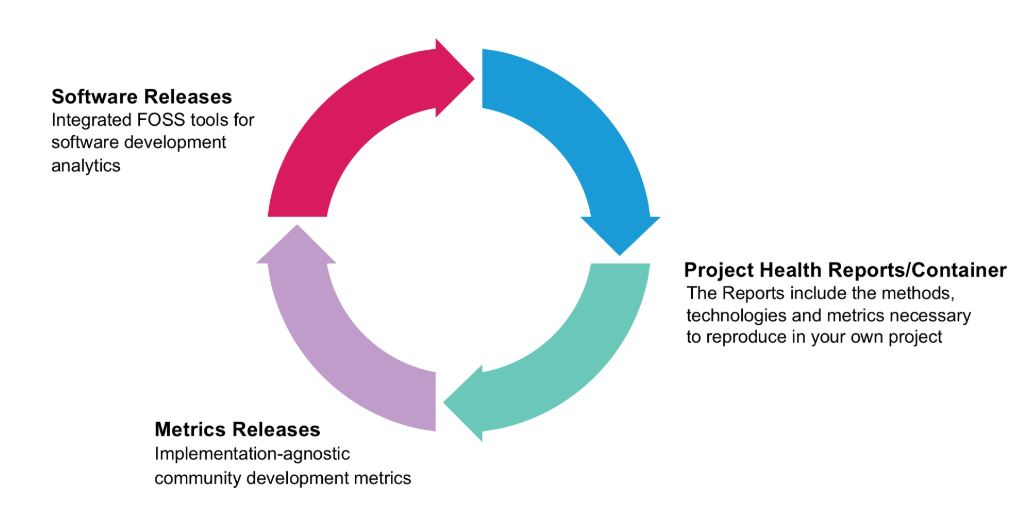
\includegraphics[width=4in,height=4.25in,clip,keepaspectratio]{images/chaossgoals.JPG}
\caption{CHAOSS Goals}
\end{figure}

These are important questions and we have come across some excellent communities and tools to help provide answers. The first project we want to highlight is CHAOSS. CHAOSS is a, "Linux Foundation project focused on creating analytics and metrics to help define community health" \cite{About}. Figure 1 shows the CHAOSS cycle for FOSS software. The project works to bring software applications to the open source community that help provide critical information about open source communities.  

One of the projects from CHAOSS is called Prospector which was open sourced by RedHat in 2017. Prospector is a tool for automated collection and continuous tracking of a wide range of metrics of open source projects that are useful in evaluating the health and trends of the project\cite{Prospector}. Prospector scores open source projects on a number of different criteria. The first rating that it computes is infrastructure. The infrastructure measurement is based on a checklist of criteria such as existing project website, mailing list, contributor licensing statement or agreement, bug tracking system, and source code repository. The second rating is on community activity. Metrics such as age of most recent release, commit activity, bug report activity, and blog posts are measured to come up with an activity score. The third measurement is one of code quality. This measurement is taken from bugs per KLOC and ratio of bugs opened to bugs closed. The last measurement is publicity. Metrics such as downloads and download frequency are collected along with number of blog posts per month and the interval at which blogs are published \cite{Open}. 

\subsection{Package Administration}
The fourth question is one of administration. What is the risk if the open source project is pulled from the internet? Is the team up to incorporating new versions of the package? Who will track the changes? How will vulnerabilities be detected and patched? A a few priorities to keep in mind with software as it pertains to software are: confidentiality, integrity, and availability. At what point will a package erode one of those three priorities? 

Khoo and Robey wrote a paper for the European Journal of Information Systems. In the paper they investigate the decision process to upgrade packaged software. The authors identify key areas that organizations should be aware of when including third-party packages that will need eventual upgrades. The first section they highlight is business needs. Business needs typically require that software is available. The business needs to software available and working. The second section the authors talk about is corporate and IT policies to mitigate software risks. What policies will be in place for what packages can be included in the software application? The next section is one on resource availability. Who is going to ensure the policies in place are followed? Who is going to patch the package? Who is going to do regression testing on the new version of the package? The last section of the authors model talks about IT needs. What are the needs of operations? Who is going to handle new system requirements when package updated require new OS packages? Overall, the authors do a good job of highlighting, from a high level, what needs to be in place for carrying out upgrades \cite{Min}

Khoo and Robey started off at the high level. McCamant and Ernst begin to focus in on solving problems caused by package upgrades. McCamant and Ernst present a "technique to assess whether replacing a component of a software system by a purportedly compatible component may change the behavior of the system" \cite{McCamant_Ernst_McCamant_Ernst_2003}. The authors want to mitigate the risk of upgrading a dependency which will break the software. They approach the problem by comparing the observed behavior of the old package to the observed behavior of a the new package and permit the upgrade only if the behaviors are compatible. They use a test suite to compare the operational abstractions of the upgrade with the old package as exercised by the application. The test suite is typically provided by the vendor on release of an update. To showcase their work they used the selection sort application. They compared one version with another and identified that the new version, through testing, used swap differently in the new version than in the old. This is interesting research, especially if we could apply it in an automated way, so that we could automate testing upgrades before incorporating the upgrades into the software.

McCamant and Ernst worked to identify what upgrades to include in a system as to not break the current system. Nguyen and Tran have provided research into identifying vulnerable software packages by using dependency graphs. When software engineers include third-party packages in their software projects they don't just include the package. They include the packages\' dependencies as well. This raises some serious concerns. How would the software engineer know that the package they just included has vulnerable dependencies? Nguyen and Tran attempt to solve this issue. They come up with a vulnerability prediction model where they used classification, are you vulnerable, and a ranking, how likely you are vulnerable. They go on to discuss precision and recall and they explain how a good prediction model should obtain high precision and recall. They also explained how it seems that the relationship between recall and precision appear to be a zero-sum game. If recall is good then precision probably is not. If precision is good then recall probably is not. 

\[Recall = \frac{TP}{TP + FN}\]
\[Precision = \frac{TP}{TP + FP}\]
\[Acc = \frac{TP + TN}{TP + TN + FP + FN}\]

The authors used static code analysis to loop over a packages dependency graph and then compare the dependency to known vulnerability databases such as MFSA, Bugzilla, and the National Vulnerability Database. As the dependencies are compared to known vulnerabilities a score would come back \cite{Nguyen_Tran_2010}.

We do not know if the research provided by Nguyen and Tran was used in industry but there are providers that will traverse dependency trees from source code repositories and notify software engineers when there are known vulnerabilities in packages included in their projects. One of these services is called Snyk. 

Snyk ties in to popular source code repositories such as GitHub and BitBucket. The application maps the full application dependency tree, finds vulnerabilities in all of the open source dependencies, continuously tests for newly disclosed vulnerabilities, and tests dependencies against a vulnerability database. When a vulnerability is detected Snyk has the ability to generate a pull request against the project to update the dependency that has the vulnerability to a version that has patched the issue. It also has the ability to send alerts via email and chat to notify developers when there is a security vulnerability \cite{Continuously}. 

Sabetta and Bezzi from the SAP Security Research wrote a paper on an approach that uses machine learning to analyze source code repositories and identify commits that are likely to fix a vulnerability. With Snyk the company leverages preexisting databases to compare dependencies against to highlight vulnerabilities. Sabetta and Bezzi propose taking it a step closer to the source code by using static code analysis on commit messages. The authors gather commit messages and classify the different messages into two categories, log and patch. They used machine learning algorithms and natural language processing methods to identify and group the different commit messages. The patch messages are important and from these messages the authors are able to come up with a certain level of precision that the package was patched to fix bug \cite{Sabetta_Bezzi_2018}. We find this approach interesting and bundled with some of the other research in this survey paper might be able to further the state of the art for bug detection. 

NPM has made headlines lately for security issues. Back in May, it removed a package called GetCookies from the NPM repository. Snyk and the research done by Sabetta and Bezzi most likely would not have caught this particular security issue. A project contributor had, on purpose, tried to hide a backdoor in the package. The NPM management was alerted by the project's community that there was a security issue. The impact, initially, seemed minimal. No one had downloaded the package since the backdoor was added. However, GetCookies, had been included in a popular package called Mailparser that had 66,000 downloads weekly \cite{Somebody}. Luckly the security issue was identified early and remediation happened quickly. This is why analyzing communities for trends such as community involvement is so important as we discussed earlier. 

Decan et al. presented a paper titled, "On the impact of security vulnerabilities in the npm package dependency network" at the MSR conference in May of 2018 in Gothenburg, Sweden. In the paper the authors present an empirical study of nearly 400 security repos over a 6-year period in the NPM dependency network. The authors highlight that Snyk released an analysis of 430,000 websites and of those no less than 77 percent of those analyzed ran at least one front-end library with a known security vulnerability \cite{decan2018impact}.  The authors aim to answer a series of questions regarding package vulnerabilities. The first question is how many packages are known to be affected by vulnerabilities. The second question is how long do packages remain vulnerable. The third question is when are vulnerabilities discovered. The fourth question is when are vulnerabilities fixed. The last question is when are vulnerabilities fixed in dependent packages. Overall, the authors did an excellent job of identifying important questions and highlighted an area that should be of concern for software engineers as they use third-party dependencies. 

As if all of this is not enough to worry about, what will the team do when a package is removed from the source repository. This happened back in March of 2016. A developer pulled a package called left-pad \cite{Williams_tweet_btn()}. A developer named Azer Koçulu pulled 250 of his modules from NPM. NPM is a popular package manager for JavaScript projects. When he pulled left-pad along with the other 249 modules it broke some of the most visited website on the internet include Facebook and Airbnb\cite{Haney_2016}. 

There are a couple of tools that help with this exact issue in industry. The first one that we want to talk about is Artifactory. Artifactory provides a feature called remote repositories. Once a remote repository is configured, software engineers can pull artifacts from the source repository, through Artifactory, and then to the software project. By pulling in dependencies through Artifactory, Artifactory is able to cache the package \cite{Remote}. This prevents the software project from breaking if the package is removed from the source repository. 

\subsection{Package Licensing}
The fifth, and final question, question that needs to be addresses is one of licensing. Licensing affects the intellectual property rights of software. Licenses can impact organizations’ rights to sell and distribute software through copyleft and each licenses brings different restrictions as to what an organization can do with the software after it is developed. Some licenses allow organizations to do whatever they want with the code or package. This includes modifying, distributing, and selling the software. Other packages allow modifying and distributing but not selling. Some do not allow modifying or distributing. The risk to an organization if a license is not vetted or identified is that it could render, depending on the license, intellectual property rights void. 

Mustonen does an excellent job of summarizing what copyleft is and why developers should care. According to Mustonen copy left is, "To copyleft a program, the programmer, besides copyrighting the program to himself, also signs a General Public License (GPL) granting everyone the right to use, modify and distribute the program on the condition that the licensee also grants similar rights over the modifications he has made"\cite{Mustonen_2003}. 

The GPL license is an interesting license and as German et al discovered below it is one of the most popular licenses for open source projects. One of the risks associated with using the GPL license is that it caries the risks of copyleft. If an organization wants to maintain intellectual property rights it might be best not to include a project with GPL. We talk more about license identification and methods for automating such identifications.


Alspaugh et al. worked  on a project to automate the detection of software licenses by using a scheme that describes the software licenses in a formal and less ambiguous form than natural language. The authors start with a tuple of <actor, operation, action, object> for expressing a right or obligation.  They are then able to scan a software repository and, using static code analysis, follow a projects dependency tree to identify any licenses included in the dependencies. Using the approach they are able to identify and calculate the copyright rights and obligations for the systems' configuration. Currently the license trace-ability analysis tool works for such licenses as the GPL, MPL, and CTL licenses {\cite{Alspaugh_Asuncion_Scacchi_2009}}.

German et al. worked on a similar problem as Alspaugh et al. German et al attacked the problem differently using sentence-matching methods to automate detecting licenses in source code files. Instead of using tubples these authors used, essentially, regular expressions to detect licenses by-inclusion and by reference. For example the authors look at the license statement and then from there are able to identify if the license is embedded in the file. The authors describe the licensing statement in four sections. The first section is a list of copyright owners. The second section is a list of authors. The third section are the licenses that cover the file. The fourth section is made up of warranty and liability statements. If a license is not embedded in the license file with the statement then the authors have to look closer at the licensing file to see where the licenses can be found. The authors work through an empirical study and show that they are able to identify licenses with GPLv2 being the most popular license in the software they analyzed \cite{German_Manabe_Inoue_2010}.

There are other licenses that are better to use from a organizational stand point if selling and maintaing intellectual property rights software are the goals. These licenses are typically BSD, MIT, and Apache to name a few. These licenses usually allow for organizations to sell, distribute, and maintain rights to the software. 

The research highlighted in this section is important because it saves organizational rights and developer time when exploring packages to include in the software project. Automating the discovery of licenses might not seem very interesting but it has a major impact. 


\bibliographystyle{IEEEtran}
\bibliography{survey} 

% \begin{figure}
% \centering
% 
\includegraphics[width=1in,height=1.25in,clip,keepaspectratio]{images/thastings.jpg}
% \caption{Photo}
% \end{figure}

% that's all folks
\end{document}
